% Copyright 2006 by Till Tantau
%
% This file may be distributed and/or modified
%
% 1. under the LaTeX Project Public License and/or
% 2. under the GNU Free Documentation License.
%
% See the file doc/generic/pgf/licenses/LICENSE for more details.


\section{Transparency}

\label{section-transparency}


For an introduction to the notion of transparency, fadings, and
transparency groups, please consult Section~\ref{section-tikz-transparency}. 


\subsection{Specifying a Uniform Opacity}

Specifying a stroke and/or fill opacity is quite easy.

\begin{command}{\pgfsetstrokeopacity\marg{value}}
  Sets the opacity of stroking operations. The \meta{value} should be
  a number between |0| and |1|, where |1| means ``fully opaque'' and
  |0| means ``fully transparent.'' A value like |0.5| will cause paths
  to be stroked in a semitransparent way.
  
\begin{codeexample}[]
\begin{pgfpicture}
  \pgfsetlinewidth{5mm}
  \color{red}
  \pgfpathcircle{\pgfpoint{0cm}{0cm}}{10mm} \pgfusepath{stroke}
  \color{black}
  \pgfsetstrokeopacity{0.5}
  \pgfpathcircle{\pgfpoint{1cm}{0cm}}{10mm} \pgfusepath{stroke}
\end{pgfpicture}
\end{codeexample}
\end{command}


\begin{command}{\pgfsetfillopacity\marg{value}}
  Sets the opacity of filling operations. As for stroking, the
  \meta{value} should be a number between |0| and~|1|.

  The ``filling transparency'' will also be used for text and images.  
  
\begin{codeexample}[]
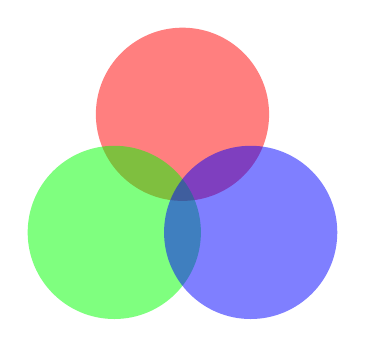
\begin{tikzpicture}
  \pgfsetfillopacity{0.5}
  \fill[red]   (90:1cm)  circle (11mm);
  \fill[green] (210:1cm) circle (11mm);
  \fill[blue]  (-30:1cm) circle (11mm);
\end{tikzpicture}
\end{codeexample}
\end{command}

Note the following effect: If you setup a certain opacity for stroking
or filling and you stroke or fill the same area twice, the effect
accumulates:

\begin{codeexample}[]
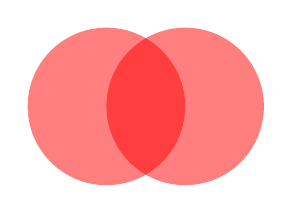
\begin{tikzpicture}
  \pgfsetfillopacity{0.5}
  \fill[red] (0,0) circle (1);
  \fill[red] (1,0) circle (1);
\end{tikzpicture}
\end{codeexample}

Often, this is exactly what you intend, but not always. You can use
transparency groups, see the end of this section, to change this.


\subsection{Specifying a Fading}

The method used by \pgfname\ for specifying fadings is quite
general: You ``paint'' the fading using any of the standard graphics
commands. In more detail: You create a normal picture, which may even
contain text, image, and shadings. Then, you create a fading based on
this picture. For this, the \emph{luminosity} of each pixel of the
picture is analysed (the brighter the pixel, the higher the luminosity
-- a black pixel has luminosity $0$, a white pixel has luminosity $1$,
a gray pixel has some intermediate value as does a red pixel). Then,
when the fading is used, the luminosity of the pixel determines the
opacity of the fading at that position. Positions in the fading where
the picture was black will be completely transparent, positions where
the picture was white will be completely opaque. Positions that have
not been painted at all in the picture are always completely
transparent.


\begin{command}{\pgfdeclarefading\marg{name}\marg{contents}}
  This command declare a fading named \meta{name} for later use. The
  ``picture'' on which the fading is based is given by the
  \meta{contents}. This \meta{contents} is normally typeset in a \TeX\
  box. The resulting box is then used as the ``picture.'' In
  particular, inside the \meta{contents} you must explicitly open a
  |{pgfpicture}| environment if you wish to use \pgfname\ commands.

  Let's start with an easy example. Our first fading picture is just
  some text:
\begin{codeexample}[]
\pgfdeclarefading{fading1}{\color{white}Ti\emph{k}Z}    

\begin{tikzpicture}
  \fill [black!20] (0,0) rectangle (2,2);
  \fill [black!30] (0,0) arc (180:0:1);
  \pgfsetfading{fading1}{\pgftransformshift{\pgfpoint{1cm}{1cm}}}
  \fill [red] (0,0) rectangle (2,2);
\end{tikzpicture}
\end{codeexample}
  What's happening here? The ``fading picture'' is mostly transparent,
  except for the pixels that are part of the word Ti\emph{k}Z. Now,
  these pixels are \emph{white} and, thus, have a high
  luminosity. This in turn means that these pixels of the fading will
  be highly opaque. For this reason, only those pixels of the big red
  rectangle ``shine through'' that are at the positions of these
  opaque pixels.

  It is somewhat counter-intuitive that the white pixels in a fading
  picture are opaque in a fading. For this reason, the color
  |pgftransparent| is defined to be the same as |black|. This allows
  one to write |pgftransparent| for completely transparent parts of a
  fading picture and |pgftransparent!0| for the opaque parts and
  things liek |pgftransparent!20| for parts that are 20\%
  transparent.

  Furthermore, the color |pgftransparent!0| (which is the same as
  white and which corresponds to completely opaque) is installed at
  the beginning of a fading picture. Thus, in the above example the
  |\color{white}| was not really necessary.

  Next, let us create a fading that gets more and more transparent as
  we go from left to right. For this, we put a shading inside the
  fading picture that has the color |pgftransparent!0| at the
  left-hand side and the color |pgftransparent!100| at the right-hand
  side. 
\begin{codeexample}[]
\pgfdeclarefading{fading2}
{\tikz \shade[left color=pgftransparent!0,
              right color=pgftransparent!100] (0,0) rectangle (2,2);}    

\begin{tikzpicture}
  \fill [black!20] (0,0) rectangle (2,2);
  \fill [black!30] (0,0) arc (180:0:1);
  \pgfsetfading{fading2}{\pgftransformshift{\pgfpoint{1cm}{1cm}}}
  \fill [red] (0,0) rectangle (2,2);
\end{tikzpicture}
\end{codeexample}

  In our final example, we create a fading that is based on a radial
  shading.
\begin{codeexample}[]
\pgfdeclareradialshading{myshading}{\pgfpointorigin}
{
  color(0mm)=(pgftransparent!0);
  color(5mm)=(pgftransparent!0);
  color(8mm)=(pgftransparent!100);
  color(15mm)=(pgftransparent!100)
}
\pgfdeclarefading{fading3}{\pgfuseshading{myshading}}

\begin{tikzpicture}
  \fill [black!20] (0,0) rectangle (2,2);
  \fill [black!30] (0,0) arc (180:0:1);
  \pgfsetfading{fading3}{\pgftransformshift{\pgfpoint{1cm}{1cm}}}
  \fill [red] (0,0) rectangle (2,2);
\end{tikzpicture}
\end{codeexample}
\end{command}

After having declared a fading, we can use it. As for shadings, there
are two different commands for using fadings:

\begin{command}{\pgfsetfading\marg{name}\marg{transformations}}
  This command sets the graphic state parameter ``fading'' to a
  previously defined fading \meta{name}. This graphic state works like
  other graphic states, that is, is persists till the end of the
  current scope or until a different transparency setting is chosen.

  When the fading is installed, it will be centered on the origin with
  its natural size. Anything outside the fading pictures's original
  bounding box will be transparent and, thus, the fading effectively
  clips against this bounding box.

  The \meta{transformations} are applied to the fading before it is
  used. They contain normal \pgfname\ transformation commands like
  |\pgftransformshift|. You can also scale the fading using this
  command. Note, however, that the transformation needs to be inverted
  internally, which may result in inaccuracies and the following
  graphics may be slightly distorted if you use a strong
  \meta{transformation}.
\begin{codeexample}[]
\pgfdeclarefading{fading2}
{\tikz \shade[left color=pgftransparent!0,
              right color=pgftransparent!100] (0,0) rectangle (2,2);}    

\begin{tikzpicture}
  \fill [black!20] (0,0) rectangle (2,2);
  \fill [black!30] (0,0) arc (180:0:1);
  \pgfsetfading{fading2}{}
  \fill [red] (0,0) rectangle (2,2);
\end{tikzpicture}
\end{codeexample}
\begin{codeexample}[]

\begin{tikzpicture}
  \fill [black!20] (0,0) rectangle (2,2);
  \fill [black!30] (0,0) arc (180:0:1);
  \pgfsetfading{fading2}{\pgftransformshift{\pgfpoint{1cm}{1cm}}
                         \pgftransformrotate{20}}
  \fill [red] (0,0) rectangle (2,2);
\end{tikzpicture}
\end{codeexample}
\end{command}

\begin{command}{\pgfsetfadingforcurrentpath\marg{name}\marg{transformations}}
  This command works like |\pgfsetfading|, but the fading is scaled
  are transformed according to the following rules:
  \begin{enumerate}
  \item
    If the current path is empty, the command has the same effect as
    |\pgfsetfading|. 
  \item
    Otherwise it is assumed that the fading has a size of 100bp times
    100bp. 
  \item
    The fading is resized and shiften (using appropriate
    transformations) such that the position
    $(25\mathrm{bp},25\mathrm{bp})$ lies at the lower-left corner of
    the current path and the position $(75\mathrm{bp},75\mathrm{bp})$
    lies at the upper-right corner of the current path.
  \end{enumerate}
  Note that these rules are the same as the ones used in
  |\pgfshadepath| for shadings. After these transformations, the
  \meta{transformations} are executed (typically a rotation).
\begin{codeexample}[]
\pgfdeclarehorizontalshading{shading}{100bp}
{ color(0pt)=(transparent!0);    color(25bp)=(transparent!0);
  color(75bp)=(transparent!100); color(100bp)=(transparent!100)}

\pgfdeclarefading{fading}{\pgfuseshading{shading}}


\begin{tikzpicture}
  \fill [black!20] (0,0) rectangle (2,2);
  \fill [black!30] (0,0) arc (180:0:1);

  \pgfpathrectangle{\pgfpointorigin}{\pgfpoint{2cm}{1cm}}
  \pgfsetfadingforcurrentpath{fading}{}
  \pgfusepath{discard}
  
  \fill [red] (0,0) rectangle (2,1);

  \pgfpathrectangle{\pgfpoint{0cm}{1cm}}{\pgfpoint{2cm}{1cm}}
  \pgfsetfadingforcurrentpath{fading}{\pgftransformrotate{90}}
  \pgfusepath{discard}

  \fill [red] (0,1) rectangle (2,2);
\end{tikzpicture}
\end{codeexample}

\end{command}

\subsection{Transparency Groups}

Transparency groups are declared using the following commands.

\begin{environment}{{pgftransparencygroup}}
  This environment should only be used inside a |{pgfpicture}|. It has
  the following effect:
  \begin{enumerate}
  \item The \meta{environment contents} is stroked/filled
    ``ignoring any outside transparency.'' This means, all previous
    transparency settings are ignored (you can still set transparency
    inside the group, but never mind). This means that if in the
    \meta{environment contents} you stroke a pixel three times in
    black, it is just black. Stroking it white afterwards yields a
    white pixel, and so on.
  \item When the group is finished, it is painted as a whole. The 
    \emph{fill} transparency settings are now applied to the resulting
    picutre. For instance, the pixel that has been painted three times
    in black and once in white is just white at the end, so this white
    color will be blended with whatever is ``behind'' the group on the
    page.
  \end{enumerate}

  Note that, depending on the driver, \pgfname\ may have to guess the
  size of the contents of the transparency group (because such a group
  is put in an XForm in \textsc{pdf} and a bounding box must be
  supplied). \pgfname\ will use normally use the size of the picture's
  bounding box at the end of the transparency group plus a safety
  margin of 1cm. Under normal circumstances, this will work nicely
  since the picture's bounding box contains everything
  anyway. However, if you have switched off the picture size tracking
  or if you are using canvas transformations, you may have to make
  sure that the bounding box is big enough. The trick is to locallly
  create a picture that is ``large enough'' and then insert this
  picture into the main picture while ignoring the size. The following
  example shows how this is done:

  
\begin{codeexample}[]
\begin{tikzpicture}
  \draw [help lines] (0,0) grid (2,2);

  % Stuff outside the picture, but still in a transparency group.
  \node [left,overlay] at (0,1) {
    \begin{tikzpicture}
      \pgfsetfillopacity{0.5}
      \pgftransparencygroup
      \node at (2,0) [forbidden sign,line width=2ex,draw=red,fill=white]
        {Smoking};
      \endpgftransparencygroup
    \end{tikzpicture}  
  };
\end{tikzpicture}
\end{codeexample}


\begin{plainenvironment}{{pgftransparencygroup}}
  Plain \TeX\ version of the |{pgftransparencygroup}| environment.
\end{plainenvironment}

\begin{contextenvironment}{{pgftransparencygroup}}
  This is the Con\TeX t version of the environment.
\end{contextenvironment}

\end{environment}



%%% Local Variables: 
%%% mode: latex
%%% TeX-master: "pgfmanual"
%%% End: 
